\documentclass[12pt,a5paper]{article}
\usepackage[margin=19mm,paperwidth=307mm,paperheight=210mm]{geometry}
\usepackage[utf8]{inputenc}
\usepackage{graphicx}
\usepackage{tikz}
\usetikzlibrary{calc}
\usepackage{fix-cm}

\def\lunghezzapagina{148.5mm}

\definecolor{mio-verde}{rgb}{0.03, 0.47, 0.19}
\parindent=0pt

\begin{document}
\pagestyle{empty}
\begin{tikzpicture}[remember picture, overlay]
\node[minimum width=\lunghezzapagina,inner sep=0pt,anchor=east, outer sep=0pt, fill opacity=1.0, align=center] at (current page.east) {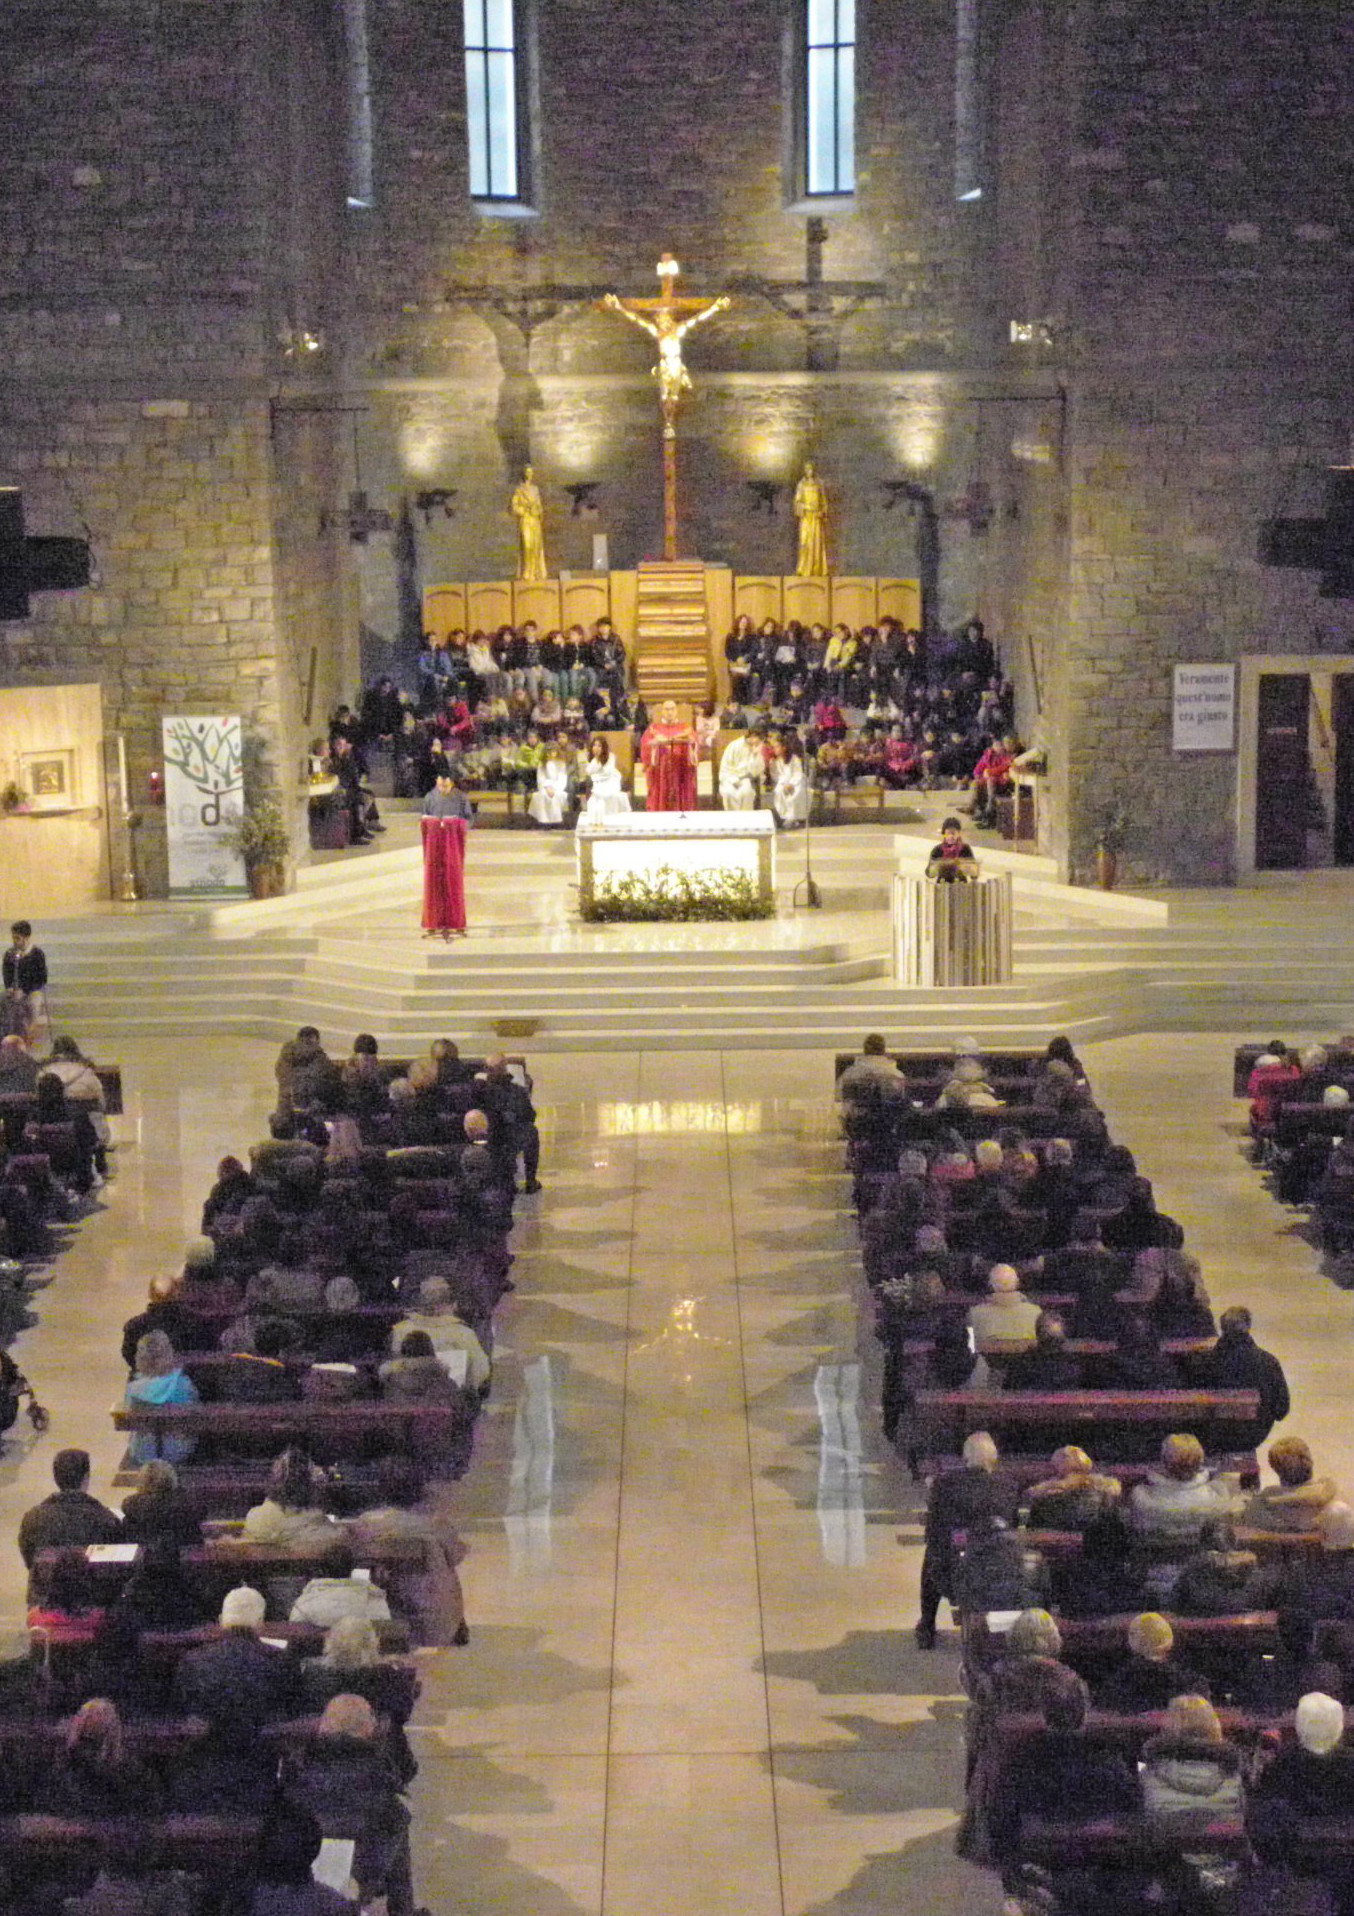
\includegraphics[width=\lunghezzapagina,height=\paperheight]{chiesa}};
\node[text width=\lunghezzapagina,anchor=north east, minimum width=\lunghezzapagina, minimum height=4.5cm, inner sep=0pt, outer sep=0pt, fill=cyan!50, fill opacity=0.7, text opacity=1, align=center] at (current page.north east) {%
\Large{\sffamily PARROCCHIA di SAN FRANCESCO in TRIESTE\par }\bigskip{\fontsize{25}{25}\selectfont\bfseries 2015: 50 ANNI di VITA\par }\bigskip LA COMUNITÀ RACCONTA\par 
};
\node [minimum width=\lunghezzapagina, anchor=south east,align=center,fill opacity=0.3] at (current page.south east) {
\includegraphics[width=8cm]{tau.png}};
\end{tikzpicture}

\end{document}
